% let's paste things we cut out from the main manuscript here, so if needed
% we can incorporate them elsewhere. Note this file is titled clipboard.tex
% for editor markup purposes, but it isn't intended to compile


\subsection{Qualitative Comparison of Scaffold-Generation Methods and Clustering}
{\bf Complete-Linkage Clustering}: As shown in \fref{clusterlanes}, the defining feature of a partitioning clustering is that every molecule maps to one and only one cluster. Thus if a chemotype is broken up among two or more clusters, using the cluster ID to map Related Molecules can retrieve only neighbors from the same cluster, ignoring the other cluster. This is not ideal for purposes of the visualization and navigation method presented here, as arbitrary neighbors would be excluded depending on how the clustering is defined.  Thus we do not advocate the use of clustering, unless it is a fuzzy clustering where all meaningful class memberships a molecule might have are considered. 

\begin{figure}
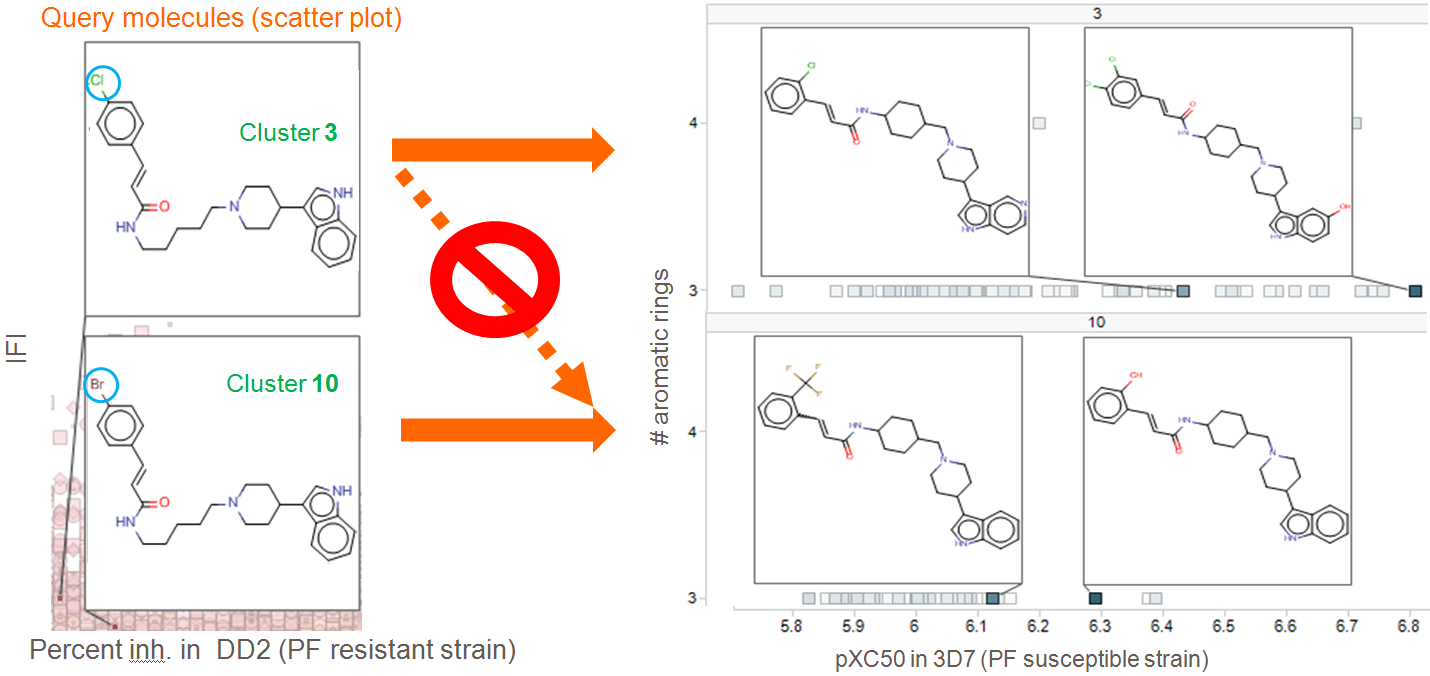
\includegraphics[width=6in]{fig/clusterlanes.png}
\caption{Illustrating one problem with clustering: bifurcation of related molecules.  When two molecules of the same chemotype differing by a halogen are split across Complete Linkage Clusters, searches of cluster neighbors for one molecule do not find its analogs in the other cluster, \ie the two related clusters are not linked.}
\label{fig:clusterlanes}
\end{figure}



{\bf NCATS R-group tool}: As opposed to the clustering method, 
if any two molecules share a common substructure that meets the standards required of a scaffold by the NCATS method (\eg being bordered by rings on each end), then those molecules will be found to contain that shared substructure as a scaffold and their activities will be used to compute aggregate properties for it. 

{\bf Other Scaffold Generation Methods}: As shown earlier, even though another scaffold generation method (represented here by the \citet{Harper2004DDclus} implementation of Frameworks) differed in its implementation details and produced different numbers of scaffolds for the same molecule, it was roughly equivalent in a qualitative sense with regard to the insights obtained. Due to substantial overlap between sets of scaffolds, ring systems responsible for activity of a molecule were generally revealed by either method. For example, the insights mentioned in \sref{scafwalk} were more or less consistent across the methods. However, there were cases where the Frameworks revealed negative information about a fragment being not important for activity that is also useful for a drug discovery scientist. For example, in \fref{frameswalk} a substructure is highlighted that is on the aggregate inactive and could be removed or substituted. This insight is not available from SSSR-based scaffolding methods such as the NCATS R-group tool since they don't define or find that fragment as a scaffold.

\begin{figure}
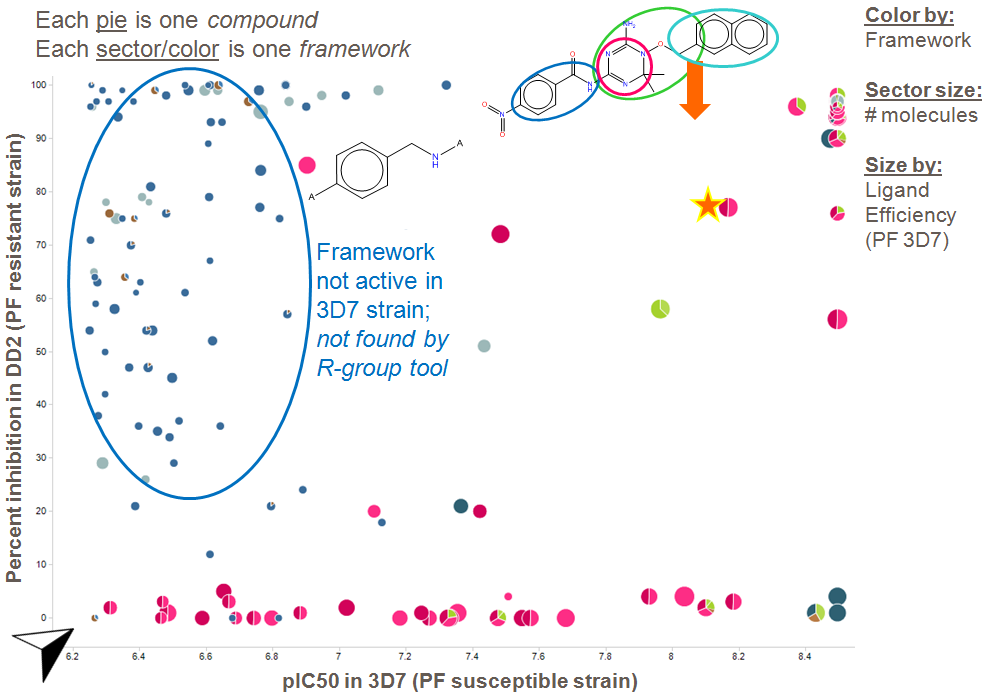
\includegraphics[width=5in]{fig/mol1_frames_scafpie.png}
\caption{Using Frameworks with the Scaffold Pies visualization. One framework is highlighted that has no equivalent in the NCATS scaffolds, but is shown to reduce activity as related molecules containing it are less active than the parent molecule.   The star symbol shows the location of the parent molecule in this Related Molecules plot, and the compass device at the origin shows the direction of favorable properties (+X and +Y axes).}      
\label{fig:frameswalk}
\end{figure}


To summarize, both multiple-scaffold decomposition methods considered in this study, \ie NCATS R-group Tool and Frameworks give comparable insights when exploring the TCAMS dataset, with some differences stemming from individual substructures that are considered shared scaffolds or not by the individual methods.  We now explore these overlaps, similarities and differences in the aggregate using the statistical methods described earlier in \sref{statmethod}.


